\ExplSyntaxOn
\cs_generate_variant:Nn \fp_set:Nn { NV }
\cs_generate_variant:Nn \fp_gset:Nn { NV }
\ExplSyntaxOff

\documentclass[12pt, a4paper, oneside]{ctexart}
\usepackage{amsmath, amsthm, amssymb, appendix, bm, graphicx, hyperref, mathrsfs, geometry, indentfirst, graphicx, diagbox}
\geometry{a4paper,left=2cm,right=2cm,top=3cm,bottom=3cm}  % 修改页边距

\usepackage{titlesec} %自定义多级标题格式的宏包
\usepackage{hyperref}
\hypersetup{hidelinks,
	colorlinks=true,
	allcolors=black,
	pdfstartview=Fit,
	breaklinks=true}
\titleformat{\section}[block]{\Large\bfseries}{\zhnum{section}.}{1em}{}[] 
% \zhum中文编号 \arabic 数字编号

\title{\vspace{-4cm}\bfseries{CH7 HOMEWORK}}
\author{\large 庞骏翔 \quad ZY2417209}  % \quad 空格一个字符 \large 小四 \bfseries 黑体
\date{}
\linespread{1.5}  % 修改行距
\setlength{\parindent}{2em} % 段首缩进两字符
\begin{document}
	
	\pagestyle{plain}
	\maketitle
	\section{1 Bundle\_Adjustment}
	
	1、文献阅读(选读1-5节)
	(1)因为BA方法其实很大程度上依赖于参数和代价函数之间的稀疏性,这种稀疏性的特殊结构可以大大降低运算的成本,提高运算的效率
	(2)3D线、旋转、投影点、平面的参数化都是非线性的,并且全局参数化是有一定约束的(例如四元数的模是1),或者是不需要内部的自由度,对于远距离的3D点,应该使用其次参数化(X,Y,Z,W),近距离的点则使用(X,Y,Z,1);对于旋转而言,由于欧拉角会存在奇异值问题,应当使用带约束的四元数以及等效旋转矢量来进行参数化(描述);误差模型的建立,平方损失函数的选择仅在高斯分布下成为ML(极大似然)或MAP(极大后验);噪声的建模很重要,噪声建模建的准,离群值就能被很好的估计,就不用使用鲁棒核函数;对于鲁棒核函数,则要限制cost函数,让其增长的不能过快
	
	类牛顿方法的优点:收敛比较快;缺点:每次迭代的步长要求较高,计算的时间较长,计算二阶导数矩阵的工作量巨大(高斯牛顿一阶近似),远离最小值时,牛顿法的收敛是十分困难的;在鞍点附近,GN法不是很理想
	
	2、BAL-dataset


	见GenetaSLAM Project homework ch7 g2oBA
	
	\section{2 直接法的Bundle Adjustment}
	
	1、数学模型
	(1)这里的任意一点自己本身是带有图像亮度信息的,这一点需要十分注意,因此这里的error就是数据集中的3D点经过投影,在图像上的到一个patch的亮度信息(16d的一个数据,当然也可以4x4),和自己本身一个patch的亮度信息之差
	(2)特别需要注意,这里的每个error是关联2个优化变量的,一个是相机的位姿,另外一个是点云的3D数据,二者同时进行优化算法的更新,所以在程序中要注意传入dynamic\_cast
	(3)这里直接使用的是g2o的自动求导(自动计算数值雅可比)功能,需要雅可比的话可以根据上面的式子求导看看
	
	2、实现
	(1)​逆深度参数化:用(μ,ν,ρ)表示,其中ρ=1/z。优势在于对远距离点的优化更稳定,特别适合单目SLAM。
	​	齐次坐标参数化:用4D齐次坐标[x,y,z,w],但需归一化(如w=1)。
	​	球坐标参数化:用(r,θ,ϕ)表示,适用于某些特殊场景(如全景相机)。
	(2)按照道理来讲,更大一些的patch可以观察更多的信息让算法受光照的影响减小(这里存在纹理的问题),但是实际上还有几何特性,我认为灰度不变假设只能停留在一定大小的局部内,超过这个局部大小,算法可能匹配到其它位置灰度相近的像素点,当然,更大的patch也意味着更大的计算量,但太小的patch又会显著受到光照的影响,因此认为patch的大小适中是较为合适的
	(3)见下图
	
	\begin{figure}[h]
		\centering
		\centerline{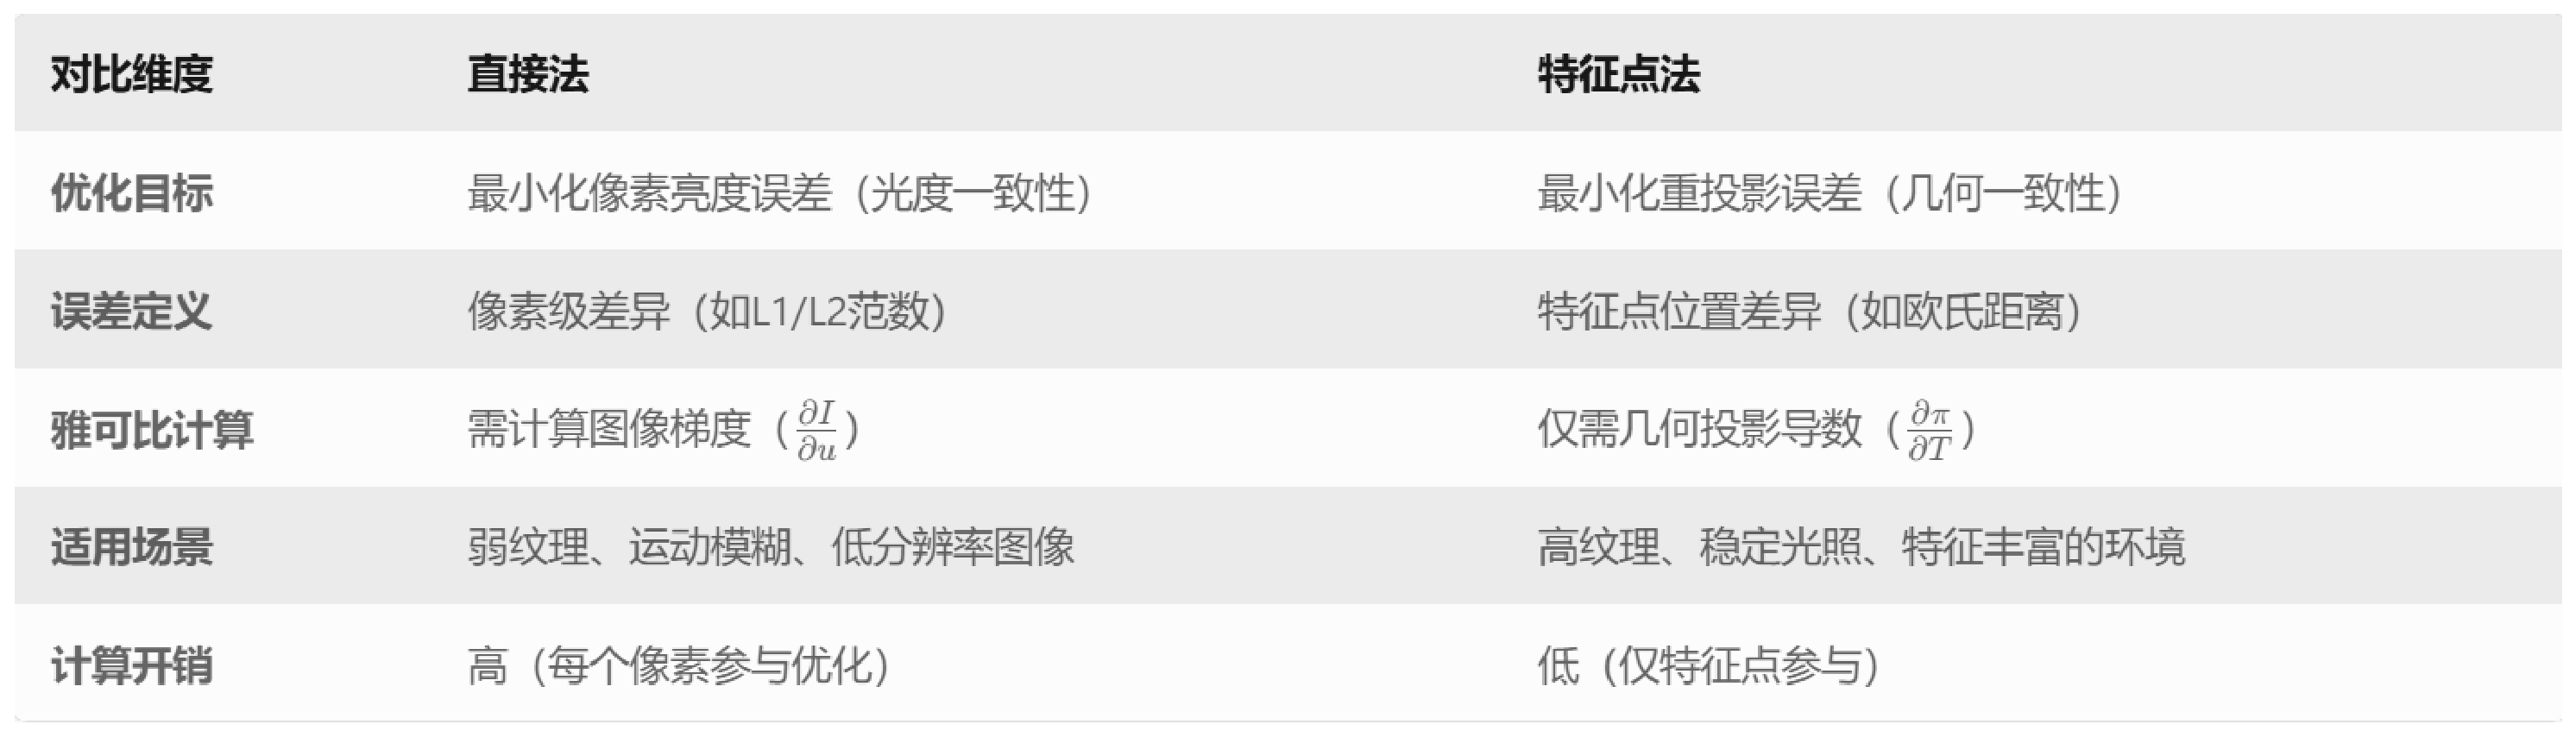
\includegraphics[scale=0.38]{特征点法直接法区别.eps}}
		\caption{特征点法直接法区别}
	\end{figure}
	 
	(4)感觉得设置初值之后看情况调整

	见GenetaSLAM Project homework ch7 directBA
	
\end{document}